\documentclass[a4paper,10pt]{article}

\usepackage[utf8]{inputenc}
\usepackage[T1]{fontenc}
\usepackage{lmodern}
\usepackage{amsmath}
\usepackage{amsfonts}
\usepackage{amssymb}
\usepackage{mathrsfs}
\usepackage{graphicx}

\usepackage{fancyhdr}
\usepackage{listings} 
\usepackage{grffile}
\usepackage{float, caption}
\usepackage{wrapfig}
\usepackage{subfig}
\usepackage{epsfig, epsf}
\usepackage{textcomp}
\usepackage{amsfonts}
\usepackage{listings}
\usepackage{eso-pic}
\usepackage{hyperref}
\usepackage[left=4cm, right=3cm, top=2.5cm, bottom=2.5cm]{geometry}  


\begin{document}

\title{Physical interpretation of the correction to Newton's
       law by Schwarzschild metric}
\author{}
\date{February 5, 2016}
\maketitle
\tableofcontents
 
\section{Introduction}

About three centuries ago, Newton formulated the Three Laws of Motion in his famous
\textit{Philosophiae naturalis principia mathematica}, and laid the foundations of what we
call now Newtonian mechanics or, since Einstein, classical mechanics. In this theory, the gravitation
is described as a force responsible for interactions between massive objects.
However, a few physical phenomena remained elusive and could not enter in the frame of Newton
theory, such as the orbit precession of Mercury. At the beginning of the twentieth century,
a new theory of gravitation came up, mainly established by Einstein, which supplanted Newton’s
law and which is still the most accurate theory of gravitation so far.
In this theory, the concept of force is totally absent and gravitation is understood as a modification
of the space-time geometry under the influence of energy and momentum coming from matter or radiation.
This modification is given by the set of ten non-linear equations known as Einstein field equations.
The Schwarzschild metric is the simpler analytical solution of these equations and describes the space-time geometry
near an homogeneous, static and isotropic spherical body as a star or a planet.
Nevertheless, we can legitimately wonder how Newton’s theory would be corrected by General Relativity.
The main goal of this project is to consider the Schwarzschild metric to figure out the correction provided by General
Relativity to Newton’s law, to give a physical interpretation of it and whenever possible,
to apply it to a concrete case like the perihelion precession of Mercury.\newline\newline
%
\textit{In our report, we use Einstein summation convention consisting of summing
on repeated indices which appears once as a subscript and once as a superscript.}\newline
\textit{Latin indices run over three spatial coordinates labels, while greek indices run
over four coordinates.}\newline
$\eta_{\mu\nu}$\textit{ denotes the Minkowski metric and we use the signature} $(+,-,-,-)$.\newline
\textit{Finally, we use natural units where }$c=1$.

\section{Bases of General Relativity}

Let us first introduce a few basic concepts, which are the basic tools of General Relativity and that we will need in the remaining
of our project. Indeed the Einstein’s theory is based on radically
different concepts than the Newton’s ones and appeals to a certain number of mathematical object, such as tensors
which were not particularly widespread at the beginning of the twentieth century.

\subsection{Equivalence principle}

The fundamental principle of General Relativity is the Equivalence Principle. We
could say that this principle emerged in the late sixtieth century when Galileo
expressed experimentally that the acceleration of an object due to gravitation is
independent of its mass.
In other words, the equivalence principle stipulates that the inertial mass $m_{I}$, which defines the ability of an object
to move further a solicitation (a force), and the gravitational mass $m_{G}$, which is a coupling coefficient between the
same object and the gravitational field\footnote{It only depends on the object features.}, are strictly equals :
%
\begin{equation}
	m_{G} = m_{I} = m
\end{equation}
%
In classical physics, there is no reason to think that these two quantities are equal.
They can be only considered as coefficients corresponding to two different physical
phenomena. However, all the experiments made so far have shown that the Equivalence Principle is accurate within an
uncertainty of magnitude $10^{-11}$ \cite{schlamminger2008test}.
By establishing the General Relativity, Einstein held this principle as true, from which follows his famous thought experiment of the elevator :
taken an observer in a closed and accelerated elevator,
there is no possibility for him to know whether the acceleration that he feels is due to a gravitational effect or to the fact that his reference
frame is non-inertial. In other words, being at rest on the surface of the Earth is equivalent to being inside
a spaceship that is being accelerated by the amount of $g$.
As a consequence, taking a reference frame $\mathcal{R}$ in presence of a static and uniform gravitational field
$\textbf{g}$, we can define a \textit{free-falling} reference frame $\mathcal{R}'$ where the gravitational field is eradicated (Fig. \ref{equivalence_illus}) and where
the laws of inertia may be applied. Indeed, applying the second law of Newton to any point $M$ in $\mathcal{R}$, we have :
%
\begin{equation}
 m\mathbf{a} = m\tfrac{\mathrm{d}^2\mathbf{OM}}{\mathrm{d}t^2} = m \mathbf{g}
\end{equation}
%
while in $\mathcal{R}'$ we have
%
\begin{equation}
 m \mathbf{a'} = m\tfrac{\mathrm{d}^2\mathbf{O'M}}{\mathrm{d}t^2}
 = m \left( \tfrac{\mathrm{d}^2\mathbf{O'O}}{\mathrm{d}t^2} + \tfrac{\mathrm{d}^2\mathbf{OM}}{\mathrm{d}t^2}\right)
 = m\left(\mathbf{a} - \mathbf{g}\right) = \mathbf{0}
\end{equation}

%
since $\mathbf{O'O} = -\frac{1}{2}\mathbf{g}t^2$.
What we did for a static and uniform gravitational field can be generalized to a time and space-dependent field
$\mathbf{g}(t,\mathbf{x})$, which allows us to reformulate the Principle of Equivalence in these words :
%
\begin{figure}
\begin{center}
\includegraphics[width=\textwidth]{equivalence_principle.pdf}
\end{center}
\caption{We can eradicate the gravitational field by defining a free-falling frame.}
\label{equivalence_illus}
\end{figure}
\begin{center}
%
\textit{In every point $M$ of a gravitational field and at any time, it exists a reference frame of coordinate $\left\{\xi^\alpha\right\}$ locally
inertial in which the laws of Nature are
identical from those that exist in an inertial reference frame in absence of gravitation.}
\end{center}
%
The next step to cross is to make the analogy with differential geometry which states that near from any point
of a non-euclidean surface we can locally erect an euclidean coordinate system.
A straightforward example is that for someone on the Earth, looking around, Earth seems to be flat (Euclidean plan) but we know that it is spherical.
The case of interest for us would be rather Minkowskian coordinate system rather than Euclidean. Nevertheless, it can be generalized to this particular
case\footnote{The underlying mathematical structure is called a pseudo-Riemannian manifold.}.
This means that gravitation can be considered as a modification of space-time.
This principle involves several important facts that built the General Relativity theory:
%
\begin{itemize}
%
\item Gravitation is described by a metric theory. The effects of the gravitation depend only on the space-time metric coefficients as well as its derivatives.
\item The co-moving frame of an object in free-fall is a local frame of reference
in which the gravitation has been canceled out : there is always a local Minkowskian frame of reference for an isolated experience.
\item In a curved space-time, the world line (trajectory) of an inertial object is no longer a
straight line but the path that minimizes the distance between two points\footnote{It is a generalization of the straight line
for curved spaces where straight line is not necessary the shortest path between two points.}. Such a world line is called a geodesic.
%
\end{itemize}

\subsection{Geodesic equation}

Let consider a particle only under the influence of gravitational forces. According to the
Principle of Equivalence above, we can find a local inertial frame $\left\{\xi^\alpha\right\}$
where its equation of motion is a straight line in space-time :
%
\begin{equation}\label{geodesic_lif}
	\frac{\mathrm{d}^2\xi^\alpha}{\mathrm{d}\tau^2} = 0
\end{equation}
%
with d$\tau$ the proper time which expresses as :
%
\begin{equation}\label{proper_time1}
	\mathrm{d}\tau^2 = \eta_{\alpha\beta}\mathrm{d}\xi^\alpha\mathrm{d}\xi^\beta
\end{equation}
%
Now we take an other system of coordinates system $x^\mu$, which may be Cartesian coordinates
as spherical coordinates or whatever. The coordinates of the local inertial frame are 
consequently functions of $x^\mu$, that is $\xi^\alpha\left(x^\mu\right)$. So by basic
calculus, equation \eqref{geodesic_lif} becomes :
%
\begin{equation}
	\frac{\partial\xi^\alpha}{\partial x^\mu} \frac{\mathrm{d}^2x^\mu}{\mathrm{d}\tau^2}
	+ \frac{\partial^2\xi^\alpha}{\partial x^\mu \partial x^\nu}
	\frac{\mathrm{d}x^\mu}{\mathrm{d}\tau}\frac{\mathrm{d} x^\nu}{\mathrm{d}\tau} = 0
\end{equation}
%
Multiplying this by $\frac{\partial x^\lambda}{\partial \xi^\alpha}$ and using the rule :
%
\begin{equation}\label{product_rule}
	\frac{\partial\xi^\alpha}{\partial x^\mu}\frac{\partial x^\lambda}{\partial \xi^\alpha}
	= \delta^\lambda_\mu
\end{equation}
%
Finally gives us the geodesic equation :
%
\begin{equation}\label{formula:geodesic}
	\frac{\mathrm{d}^2x^\lambda}{\mathrm{d}\tau^2} + \Gamma^\lambda_{\mu\nu} 
	\frac{\mathrm{d}x^\mu}{\mathrm{d}\tau}\frac{\mathrm{d}x^\nu}{\mathrm{d}\tau} = 0
\end{equation}
%
where $\Gamma^\lambda_{\mu\nu}$ are called Christoffel symbols.
They are defined by :
%
\begin{equation}\label{affine_connection}
	\Gamma^\lambda_{\mu\nu} = \frac{\partial x^\lambda}{\partial \xi^\alpha}
	\frac{\partial^2\xi^\alpha}{\partial x^\mu \partial x^\nu}
\end{equation}
%
and we note that they are symmetric in the lower two indices.
The proper time $\mathrm{d}\tau$ may also be expressed in the new coordinate system :
%
\begin{equation}\label{proper_time2}
	\mathrm{d}\tau^2 = \eta_{\alpha\beta} \frac{\partial \xi^\alpha}{\partial x^\mu}
	\mathrm{d}x^\mu \frac{\partial \xi^\beta}{\partial x^\nu} \mathrm{d}x^\nu
\end{equation}
%
From here we introduce the metric tensor $g$ which the components are :
%
\begin{equation}\label{metric1}
	g_{\mu\nu} = \eta_{\alpha\beta} \frac{\partial \xi^\alpha}{\partial x^\mu}
	\frac{\partial \xi^\beta}{\partial x^\nu}
\end{equation}
%
and which are symmetric. As Minkowski metric in the case of special relativity,
it allows us to raise or to lower indices of a vector or a tensor by contraction :
%
\begin{equation}
 A_\mu = g_{\mu\nu} A^\nu \quad \mathrm{and} \quad A^\mu = g^{\mu\nu} A_\nu
\end{equation}
%
where $g^{\mu\nu}$ is the inverse of the metric tensor defined as :
%
\begin{equation}
	g_{\mu\lambda}g^{\lambda\nu} = \delta^\nu_\mu
\end{equation}
%
Finally, equation \eqref{proper_time2} may be expressed as :
%
\begin{equation}\label{invariant}
	\mathrm{d}\tau^2 = g_{\mu\nu}\mathrm{d}x^\mu\mathrm{d}x^\nu
\end{equation}
%
Geodesic equation is only available for massive particles. In fact, this cannot be use for
massless particles as photons because in this case, the right-hand side of
\eqref{proper_time1} vanishes. Nevertheless, calculus may be done by replacing $\tau$ in
\eqref{geodesic_lif} by any parameter, as $\sigma = \xi^0$ for example. In the remaining of the report,
we are going to restrict us only to massive particles.

\subsection{Christoffel symbols}

We have seen that Christoffel symbols and the metric tensor appeared naturally when we want to
express the equation of motion in an arbitrary coordinate system. Now we are going to see the
link between these two objects and thus the link between Christoffel symbols and the
structure of space-time, that is the metric.
For this aim, we have first to differenciate the metric tensor with respect to $x^\lambda$,
which gives :
%
\begin{equation}\label{equation_longue}
	\frac{\partial g_{\mu\nu}}{\partial x^\lambda} = 
	\eta_{\alpha\beta}\left(\frac{\partial^2 \xi^\alpha}{\partial x^\lambda\partial x^\mu}
	\frac{\partial \xi^\beta}{\partial x^\nu} +
	\frac{\partial \xi^\alpha}
	{\partial x^\mu}\frac{\partial^2\xi^\beta}{\partial x^\lambda \partial x^\nu}\right)
\end{equation}
%
To go further we need an extra relation which may be obtain by multiplying
\eqref{affine_connection} by $\frac{\partial \xi^\beta}{\partial x^\lambda}$ and by using
\eqref{product_rule}. That gives us :
%
\begin{equation}
	\frac{\partial^2 \xi^\alpha}{\partial x^\mu \partial x^\nu}
	= \Gamma^\lambda_{\mu\nu} \frac{\partial \xi^\alpha}{\partial x^\lambda}
\end{equation}
%
This relation allows to express \eqref{equation_longue} with Christoffel symbols :
%
\begin{equation}
	\frac{\partial g_{\mu\nu}}{\partial x^\lambda} = 
	\eta_{\alpha\beta}\left(\Gamma^\rho_{\lambda\mu}
	\frac{\partial\xi^\alpha}{\partial x^\rho}
	\frac{\partial \xi^\beta}{\partial x^\nu} + \Gamma^\rho_{\lambda\nu}
	\frac{\partial\xi^\alpha}{\partial x^\mu}
	\frac{\partial \xi^\beta}{\partial x^\rho}\right)
\end{equation}
%
Using \eqref{metric1}, we find :
%
\begin{equation}\label{equation_derive_metrique}
	\frac{\partial g_{\mu\nu}}{\partial x^\lambda} =
	\Gamma^\rho_{\lambda\mu}g_{\rho\nu} + \Gamma^\rho_{\lambda\nu}g_{\mu\rho}
\end{equation}
%
We recall that $\Gamma^\lambda_{\mu\nu}$ and $g_{\mu\nu}$ are symmetric under permutation of
$\mu$ and $\nu$. So by adding to \eqref{equation_derive_metrique} the same equation with
$\mu$ and $\lambda$ interchanged and by subtracting the same equation with $\nu$ and
$\lambda$ interchanged, we obtain :
%
\begin{equation}
\begin{aligned}
	\frac{\partial g_{\mu\nu}}{\partial x^\lambda}
	+ \frac{\partial g_{\lambda\nu}}{\partial x^\mu}
	- \frac{\partial g_{\mu\lambda}}{\partial x^\nu}
	& = g_{\sigma\nu} \Gamma^\sigma_{\lambda\mu} 
	+ g_{\sigma\mu} \Gamma^\sigma_{\lambda\nu} 
	+ g_{\sigma\nu} \Gamma^\sigma_{\mu\lambda} 
	+ g_{\sigma\lambda} \Gamma^\sigma_{\mu\nu} 
	- g_{\sigma\lambda} \Gamma^\sigma_{\nu\mu} 
	- g_{\sigma\mu} \Gamma^\sigma_{\nu\lambda} \\
	& = 2g_{\sigma\nu}\Gamma^\sigma_{\mu\lambda}
\end{aligned}
\end{equation}
%
Finally, we multiply each term by $g^{\nu\rho}$ an obtain the expected equation :
%
\begin{equation}\label{formula:christoffel}
	\Gamma^\sigma_{\mu\nu} =
	\frac{1}{2}g^{\sigma\lambda}\left\{\frac{\partial g_{\lambda\nu}}{\partial x^\mu}
	+ \frac{\partial g_{\mu\lambda}}{\partial x^\nu}
	- \frac{\partial g_{\mu\nu}}{\partial x^\lambda}\right\}
\end{equation}
%
Not only this relation gives the link between Christoffel symbols and geometrical structure
of space-time but also it provides a useful expression to compute these symbols. In fact, the
expression \eqref{affine_connection} leads to laborious calculus but adding properties
of symmetries of the symbols to relation \eqref{formula:christoffel}, these calculus are more easier as we will see later.
Moreover, we want to indicate that Christoffel symbols are not tensors. If it were the case,
since they are null in the good frame (a local inertial one), we might deduce by a change of frame
that they are null in all frames. By the way, in General Relativity we are no longer restricted to Lorentz transformation
in a change of frame but to any\footnote{That is the reason why \textit{General} Relativity.} diffeomorphism
$x^\mu \rightarrow {x'}^\nu$ and so components of a vector $\textbf{A}$ transform as :
%
\begin{equation}
 {A'}^\mu = \frac{\partial {x'}^\mu}{\partial x^\nu} A^\nu \quad \mathrm{and} \quad {A'}_\mu = \frac{\partial x^\nu}{\partial {x'}^\mu} A_\nu
\end{equation}

\subsection{Einstein field equations}

Before introducing the Einstein field equations that allows to determine the metric tensor $g_{\mu\nu}$ from the repartition of mass
and energy, we will need to introduce few more quantities that intervene in its expression.

\subsubsection{Ricci tensor}

The Ricci tensor, denoted $R_{\mu\nu}$, is a symmetric tensor and it is related to the Christoffel symbols by the
equation\footnote{To see a proof of this relation, see \cite{weinberg1972gravitation}
or whichever textbook on General Relativity.} :
%
\begin{equation}
 R_{\mu\nu}=\partial_\nu \Gamma^{\sigma}_{\mu\sigma}-
\partial_\sigma\Gamma^{\sigma}_{\mu\nu}+
\Gamma^{\rho}_{\mu\sigma}\Gamma^{\sigma}_{\rho\nu}
-\Gamma^{\rho}_{\mu\nu}\Gamma^{\sigma}_{\rho\sigma}
\end{equation}
%
where $\partial_\mu$ is a shorthand for $\frac{\partial}{\partial x^\mu}$.
Its contraction gives us what we call the scalar curvature $R$ :
%
\begin{equation}
 R = {R^\lambda}_\lambda = g^{\mu\lambda}R_{\mu\lambda}
\end{equation}
%

\subsubsection{Stress-energy tensor}

The stress-energy tensor, denoted $T_{\mu\nu}$ describes the repartition of mass and energy in space-time,
which is the source of the gravitational field. As the Ricci tensor, it is symmetric.
For an ideal gas, its expression is :
%
\begin{equation}
 T^{00} = \rho, \quad T^{0i} = 0 \quad  \mathrm{and} \quad T^{ij} = P\delta^{ij}
\end{equation}
%
where $\rho$ and $P$ are respectively the mass-energy density and the pressure of the gas.
Because we will exclusively work in empty space in the next of the report, it will be taken null.
Nevertheless, we needed to introduce it to give the general expression of Einstein equations.

\subsubsection{Einstein equations}

Now that we have all the prerequisites, we can introduce the Einstein field equations, which are given in the form of tensor
equations\footnote{To have a proof, see previous footnote} by :
%
\begin{equation}\label{Einstein}
	R_{\mu\nu}-\frac{1}{2}g_{\mu\nu}R=8\pi G T_{\mu\nu}
\end{equation}
%
The field equations are non-linear and as the tensors are all symmetric,
there are six independent equations that determine the expression of the metric tensor.
For the general case, we can just make them resolved by
using approximation methods or by using numerical methods. But there are also some
particular cases where the field equations can be solved analytically :
the Schwarzschild metric is one of them.
Finally, by multiplying these equations by $g^{\nu\mu}$, we obtain a relation between $R$ and $T_{\mu\nu}$ :
%
\begin{equation}\label{scalar_curvature_stress_energy}
 R = - 8\pi G {T^\lambda}_\lambda
\end{equation}


\section{Schwarzschild metric}

Here we are going to study the Schwarzschild metric, which is an analytical solution to
the Einstein field equations in the static isotropic case. We will need some symmetric views and
tensorial calculus to arrive at its expression.

\subsection{The general static isotropic metric}

We are going to find the most general metric tensor that can represent a static isotropic
gravitational field. The symmetry arguments are essential. 

We consider the invariant proper time in spherical coordinates :
%
\begin{equation}\label{minkowski_spherical}
	\mathrm{d}\tau^2 = \mathrm{d}t^2-\mathrm{d}r^2-r^2(\mathrm{d}\theta ^2+\sin^2\theta
	\mathrm{d}\phi^2)
\end{equation}
%
The term $\mathrm{d}\theta ^2+\sin^2\theta \mathrm{d}\phi^2$ has symmetric and isotropic
characteristics.
We can generalize it to an equation for any spherically symmetric metric :
%
\begin{equation}
	\mathrm{d}\tau^2=A\mathrm{d}t^2-B\mathrm{d}t\mathrm{d}r-Cr^2-D(\mathrm{d}\theta ^2
	+\sin^2\theta \mathrm{d}\phi^2)
\end{equation}
%
where $A$, $B$, $C$ and $D$ are functions of the coordinates.
For symmetric and isotropic reasons, these functions cannot depend on $\theta$
or $\phi$. And since we expect the symmetry under the transformation $\phi$ $\rightarrow$
$-\phi$ and $\theta$ $\rightarrow$ $\pi-\theta$, there are no cross terms such
$\mathrm{d}r\mathrm{d}\theta$ or $\mathrm{d}\phi \mathrm{d}t$.

We define a new radial coordinate $r'$ such that $\left(r'\right)^2=D$ :
%
\begin{equation}
	\mathrm{d}\tau^2=A'(t,r')\mathrm{d}t^2-B'(t,r')\mathrm{d}t\mathrm{d}r'-C'(t,r')r'^2-\left(r'\right)^2
	\left(\mathrm{d}\theta ^2+\sin^2\theta \mathrm{d}\phi^2\right)
\end{equation}
%
and we can finally transform the time coordinate :
%
\begin{equation}
	\mathrm{d}t'=f\mathrm{d}t+g\mathrm{d}r'
\end{equation}
%
with f and g arbitrary functions\footnote{We are free to measure time as we want.}. This can allow us to eliminate the cross term
$\mathrm{d}r'\mathrm{d}t$ \footnote{This can be seen as diagonalization of the matrix $g_{\mu\nu}$.}.
At last, we apply the static condition and know that $A'$ and $B'$ do not depend on $t'$.
Finally, by leaving quotes aside, we have :
\begin{equation}\label{symmetry}
	\mathrm{d}\tau^2=A\left(r\right)\mathrm{d}t^2-B\left(r\right)
	\mathrm{d}r^2-r^2\mathrm{d}\theta ^2-r^2\sin^2\theta \mathrm{d}\phi^2
\end{equation}

This is the standard form of an static isotropic metric.

\subsection{Derivation of the Schwarzschild metric}

To get the Schwarzschild metric, that is by determining the functions $A$ and $B$, we apply the Einstein field equations \eqref{Einstein} to the general
static isotropic metric \eqref{symmetry}.

By definition, Schwarzschild metric describes structure of space-time outside a spherical, neutral and non-rotating mass in an empty space. Then, as we said previously, the
stress-energy tensor $T_{\mu\nu}$ is null and according to \eqref{scalar_curvature_stress_energy}, so as the scalar curvature. In this case, Einstein
field equations \eqref{Einstein} reduces to $R_{\mu\nu}=0$.

In order to find components of the Ricci tensor, we need to calculate the Christoffel symbols
$\Gamma^{\sigma}_{\mu\nu}$ from the metric $g_{\mu\nu}$. So first we need to identify the
metric components from equation \eqref{symmetry} using \eqref{invariant}. For the components
of $g_{\mu\nu}$, we label $x^0=t$, $x^1=r$, $x^2=\theta$, $x^3=\phi$ then :
%
\begin{equation}
g_{\mu\nu}=\left(
	\begin{array}{cccc}
	g_{00} & g_{01} & g_{02} & g_{03}\\
	g_{10} & g_{11} & g_{12} & g_{13}\\
	g_{20} & g_{21} & g_{22} & g_{23}\\
	g_{30} & g_{31} & g_{32} & g_{33}\\
	\end{array}
\right)=\left(
	\begin{array}{cccc}
	g_{tt} & g_{tr} & g_{t\theta} & g_{t\phi}\\
	g_{rt} & g_{rr} & g_{r\theta} & g_{r\phi}\\
	g_{\theta t} & g_{\theta r} & g_{\theta\theta} & g_{\theta\phi}\\
	g_{\phi t} & g_{\phi r} & g_{\phi\theta} & g_{\phi\phi}\\
		\end{array}
\right)
\end{equation}

Consequently, non-vanishing elements of the metric
$g_{\mu\nu}$ and its inverse $g^{\mu\nu}$ are :
%
\begin{equation}
	g_{00}=A\left(r\right),	\qquad g^{00}=1/A\left(r\right)
\end{equation}
%
\begin{equation}
	g_{11}=-B\left(r\right),\qquad g^{11}=-1/B\left(r\right)
\end{equation}
%
\begin{equation}
	g_{22}=-r^2,\qquad g^{22}=-1/r^2
\end{equation}
%
\begin{equation}
	g_{33}=-r^2\sin^2\theta,\qquad g^{33}=-1/\left(r^2\sin^2\theta\right)
\end{equation}

Now we can apply the formula \eqref{formula:christoffel} and calculate the Christoffel
symbols $\Gamma^{\sigma}_{\mu\nu}$. We recall that Christoffel symbols are symmetric by
interchanging $\mu$ and $\nu$. The non-vanishing components are :
%
\begin{equation}\label{christoffel}
	\Gamma^{0}_{01}=A'/\left(2A\right),\qquad \Gamma^{1}_{00}=A'/\left(2B\right),
	\qquad \Gamma^{1}_{11}=B'/\left(2B\right)
\end{equation}
%
\begin{equation}
	\Gamma^{1}_{22}=-r/B,\qquad \Gamma^{1}_{33}=-\left(r\sin^2\theta\right) /B,
	\qquad \Gamma^{2}_{12}=1/r
\end{equation}
%
\begin{equation}
	\Gamma^{2}_{33}=-\sin\theta \cos\theta ,\qquad \Gamma^{3}_{13}=1/r,
	\qquad \Gamma^{3}_{23}=\cot\theta
\end{equation}

Now we substitute the expression of $\Gamma^{\sigma}_{\mu\nu}$ into $R_{\mu\nu}$. Only the diagonal
components are non-vanishing :
%
\begin{equation}
	R_{00}=-\frac{A''}{2B}+\frac{A'}{4B}\left(\frac{A'}{A}+\frac{B'}{B}\right)-\frac{A'}{rB}
\end{equation}
%
\begin{equation}
	R_{11}=\frac{A''}{2A}-\frac{A'}{4A}\left(\frac{A'}{A}+\frac{B'}{B}\right)-\frac{B'}{rB}
\end{equation}
%
\begin{equation}\label{R22}
	R_{22}=\frac{1}{B}-1+\frac{r}{2B}\left(\frac{A'}{A}-\frac{B'}{B}\right)
\end{equation}
%
\begin{equation}
	R_{33}=R_{22}\sin^2\theta
\end{equation}
%
(A prime means differentiation with respect to $r$).
The fourth equation is merely the consequence of the first three. From these equations, we can establish the relation :
%
\begin{equation}
	A'B+AB'=0
\end{equation}
%
In other words, $AB$=constant. By imposing the boundary condition that when $r\rightarrow \infty$ the metric tensor must approach
the Minkowski metric \eqref{minkowski_spherical}, we have $A(r)\rightarrow 1$ and $B(r) \rightarrow 1$. Then the constant of integration is equal to $1$.
Now, substituting this relation into \eqref{R22}, we get :
%
\begin{equation}
	\frac{\mathrm{d}\left(rA\right)}{\mathrm{d}r}= 1
\end{equation}

By integrating this equation, we can find easily :
%
\begin{equation}\label{function_A_and_B}
	A\left(r\right) = 1 + \frac{k}{r} \quad \mathrm{and}
	\quad B\left(r\right) = \left(1+\frac{k}{r}\right)^{-1}
\end{equation}

where $k$ is an integration constant.

Far from the mass, we can place us in weak field approximation, that is $g_{\mu\nu} = \eta_{\mu\nu} + h_{\mu\nu}$ with $\left| h_{\mu\nu}\right| \ll 1$. In
this limit and for any metric, we have the relation\footnote{See \cite{weinberg1972gravitation}.} $g_{00} = 1 + 2\phi$ where $\phi = -\frac{GM}{r}$ is
the classical gravitational field.
Considering this limit we find that $k=-2GM$ so injecting this expression in \eqref{function_A_and_B}, we find that
$A(r) = 1 - \frac{2GM}{r}$ and $B(r) = \left( 1-\frac{2GM}{r}\right)^{-1}$. Finally we obtain the Schwarzschild metric :
%
\begin{equation}\label{schwa}
	\mathrm{d}\tau^2=\left(1-\frac{2GM}{r}\right)\mathrm{d}t^2
	-\left(1-\frac{2GM}{r}\right)^{-1}\mathrm{d}r^2-r^2\left(\mathrm{d}\theta ^2
	+\sin^2\theta \mathrm{d}\phi^2\right)
\end{equation}
%
As the Schwarzschild metric describes static isotropic
gravitational field, it is a good candidate to describe the movement of the planets. In the next part so, by
applying this metric we will search for a correction term in Newton's law brought by General Relativity.

\section{Correction to the Newton's law}

In this section, we will first recall the expression of the total energy of a test particle of mass $m$ in a central force field
generated by a mass $M$. Then we will derive an equivalent expression in the relativistic case. To do so, we will start
from the geodesic equation of the test particle in the Schwarzschild metric due to the presence of the mass $M$. Then comparing
the two expression we will deduce the corrective term.

\subsection{Central force field in classical mechanics}

Let us consider the motion of a test particle of mass $m$ in central force field, $\textbf{F}(\textbf{r}) = f(r)\textbf{e}_r$
with the origin as its force center. The force derives from a potential energy $V(r)$ which is function of $r$ alone and then the Lagrangian
associated to the problem is $\mathcal{L} = T - V = \frac{1}{2}m v^2 - V(r)$. In polar coordinates, the velocity has for expression
$\mathbf{v}= \dot{r}\mathbf{e}_r + r\dot{\theta} \mathbf{e}_\theta$, then the expressions of the Lagrangian becomes :
%
\begin{equation}
 \mathcal{L} = \frac{1}{2}m\left(\dot{r}^2 + r^2 \dot{\theta}^2\right) - V(r)
\end{equation}
%
Using the Euler-Lagrange equations : 
%
\begin{equation}
 \frac{\mathrm{d}}{\mathrm{d}t}\left( \frac{\partial \mathcal{L}}{\partial \dot{q}_i} \right) = \frac{\partial \mathcal{L}}{\partial q_i}
\end{equation}
%
we obtain :
%
\begin{equation}\label{conservation_1}
  \frac{\mathrm{d}}{\mathrm{d}t}\left( mr^2\dot{\theta}\right) = 0
\end{equation}
%
\begin{equation}\label{conservation_2}
   m\ddot{r} - mr\dot{\theta}^2 = -\frac{\partial V(r)}{\partial r}
\end{equation}
%
The first equation is easy to integrate and we obtain a conserved quantity $mr^2\dot{\theta} = J$.
It is nothing else than the magnitude of the angular momentum vector $ \mathbf{J} = \mathbf{r} \times \mathbf{p}$.
Now injecting this relation in \eqref{conservation_2} and integrating, we obtain a second conserved quantity which is the total energy
of the system :
%
\begin{equation}
 E = \frac{1}{2}m\dot{r}^2 + \frac{1}{2}\frac{J^2}{mr^2} + V(r)
\end{equation}
%
In our particular case, we have $V(r) = - \frac{2GmM}{r}$ and normalizing the expression by the mass $m$ of the test particle, we obtain :
%
\begin{equation}\label{classical_relation}
  e = \frac{1}{2}\dot{r}^2 + \frac{1}{2}\frac{h^2}{r^2} -\frac{2GM}{r}
\end{equation}
%
where $e = E/m$ and $h=J/m$.

\subsection{Relativistic case and corrective term}

First, we have to derive geodesic equation for the test particle. In this objective, we inject expression of the Christoffel symbols
\eqref{christoffel} in \eqref{formula:geodesic}. We find :
%
\begin{subequations}\label{schwarz_geodesic}
  \begin{align}
	\lambda = 0 &: \qquad \ddot{t} + \frac{A'}{A}
	\dot{t}\dot{r}
	=0 \\
	\lambda = 1 &: \qquad \ddot{r} + \frac{B'}{2B}{\dot{r}}^2 + \frac{A'}{2B}{\dot{t}}^2
	- \frac{r}{B} {\dot{\theta}}^2 - \frac{r}{B}\sin^2(\theta) {\dot{\phi}}^2
	=0 \\
	\lambda = 2 &: \qquad \ddot{\theta} + \frac{2}{r}\dot{r}\dot{\theta}
	- \sin(\theta)\cos(\theta){\dot{\phi}}^2
	= 0 \\
	\lambda = 3 &: \qquad \ddot{\phi} + \frac{2}{r}\dot{r}\dot{\phi} + 2\cot(\theta)\dot{\theta}\dot{\phi}
	=0
  \end{align}
\end{subequations}
%
where dot means differentiation with respect to $\tau$ and prime holds for differentiation with respect to $r$.
We now consider in the remaining of our study and without loss of generality (since the field is isotropic) that the movement
takes place in the plan $\theta = \frac{\pi}{2}$. So previous equations \eqref{schwarz_geodesic} become :
%
\begin{subequations}
  \begin{align}
	&\ddot{t} + \frac{A'}{A} \dot{t}\dot{r} =0 \label{machin_1} \\
	&\ddot{r} + \frac{B'}{2B}{\dot{r}}^2 + \frac{A'}{2B}{\dot{t}}^2 - \frac{r}{B}{\dot{\phi}}^2 = 0 \label{machin_2}\\
	&\ddot{\phi} + \frac{2}{r}\dot{r}\dot{\phi} = 0 \label{machin_3}
  \end{align}
\end{subequations}
%
and equation for $\lambda = 2$ is no longer pertinent.
Multiplying equation \eqref{machin_1} by $A$ and equation \eqref{machin_3} by $r^2$ we can rewrite them :
%
\begin{subequations}
\begin{align}
 &\frac{\mathrm{d}}{\mathrm{d}\tau}\left(\dot{t}A(r)\right) = 0\\
 &\frac{\mathrm{d}}{\mathrm{d}\tau}\left(r^2\dot{\phi}\right) = 0
 \end{align}
\end{subequations}
%
so the quantities :
%
\begin{subequations}
 \begin{align}
  &A(r) \dot{t} \equiv \sqrt{2e + 1}\label{conservation_energy}\\
  &r^2\dot{\phi} \equiv h \label{conservation_angular}
  \end{align}
\end{subequations}
%
are conserved along the trajectory. For the moment, $e$ can be taken as an arbitrary constant but in fact we will that it is 
the total energy of the system.
Now by introducing these relations in \eqref{machin_2} and multiplying it by $2B\dot{r}$, we can rewrite it as :
%
\begin{equation}
 \frac{\mathrm{d}}{\mathrm{d}\tau}\left(B{\dot{r}}^2 - \frac{2e+1}{A(r)} + \frac{h^2}{r^2}\right) = 0
\end{equation}
%
Then, we obtain one more conserved quantity : 
%
\begin{equation} \label{machin_4}
  B(r)\dot{r}^2 + \frac{h^2}{r^2} - \frac{2e+1}{A(r)} = k  
\end{equation}
%
But from the expression of the metric we deduce an other relation :
\begin{equation}
 1 = A(r)\dot{t}^2 - B(r) \dot{r}^2 - r^2\dot{\phi}^2 
\end{equation}
%
(we recall that $\theta = \pi/2$). After injecting relations \eqref{conservation_energy} and \eqref{conservation_angular}, previous equation becomes :
\begin{equation}
 1 = \frac{2e+1}{A(r)} - B(r) \dot{r}^2 - \frac{h^2}{r^2} = -k
\end{equation}
%
Then we see that we have $k=-1$.
Multiplying by $A$ and replacing by its expression in equation \eqref{machin_4}, we can put it in the form:
%
\begin{equation}
 e = \frac{\dot{r}^2}{2} - \frac{GM}{r} + \frac{h^2}{2r^2} - \frac{GMh^2}{r^3}
\end{equation}
%
which is the same as equation \eqref{classical_relation} excepted for the term proportional to $\frac{1}{r^3}$ which is of course 
the excepted corrective term. From this and 
reintroducing the mass $m$ of the test particle, we deduce the expression of the corrected potential energy :
%
\begin{equation}
 V_{\mathrm{corr.}}(r) = -\frac{GmM}{r} - \frac{GMJ^2}{mr^3}
\end{equation}
%
and then the expression of the corresponding force :
%
\begin{equation}
	 \mathbf{F}_{\mathrm{corr.}}(r) = - \frac{\mathrm{d}}{\mathrm{d}r} \left(V(r)\right)\mathbf{e}_r = \left[-\frac{GmM}{r^2} - \frac{3GMJ^2}{mr^4}\right] \mathbf{e}_r
\end{equation}
%
So the classical force is corrected by an attractive term proportional to $\frac{1}{r^4}$. As we will see in the next section, this term is responsible for
the precession of the perihelion of Mercury and it is because it is non negligible for short distances that this phenomena was visible only in the case of Mercury.
Now we know that it affects all the planets in solar system, included the Earth.

\section{Application}

\subsection{Perihelion precession of Mercury}

In this part we are going to apply the results that we have found to interpret the
perihelion precession of Mercury. In fact, in past hundred years, this problem
was never been explained correctly, until the appearance of the general relativity.
We start by looking for the analytic formulas and thanks to the numerical tools that we
have acquired, then we can move on to the numerical simulation to visualize the orbit of Mercury.

In Newton's classical case, most of the movements of the planet is described by the
Binet's formula:
%
\begin{equation}\label{Binet classique}
	\frac{\mathrm{d}^2u}{\mathrm{d}\phi^2}+u=\frac{GM}{h^2}
\end{equation}
%
with $u=1/r$ and $h$ the specific angular momentum with $\textbf{h}=\textbf{L}/m$.

The demonstration of the Binet's equation from the law of Newtonian movement is given in
the lecture of the course \textit{4P017 Gravitation} of the first semester. We quote the
link of the lecture here: (\url{http://syrte.obspm.fr/~souchay/cours2012/coursII.pdf}). The
complete demonstration begins from page 3.

The equation \eqref{Binet classique} can be integrated, with the demonstration in the
lecture we get:
\begin{equation}\label{orbit classique}
	u=\frac{1}{r}=\frac{GM}{h^2}\left[ 1+\sqrt{1+\frac{2h^2E}{G^2M^2m}}
	\mathrm{cos}\left( \theta-\theta_0\right)\right]
\end{equation}
%
with $E$ the total energy of the planet. We can also write it in this form:
%
\begin{equation}
	r=\frac{1}{u}=\frac{p}{1+e\mathrm{cos}\left( \theta-\theta_0\right) }
\end{equation}
%
with $p=\frac{h^2}{GM}$ and the eccentricity $e=\sqrt{1+\frac{2h^2E}{G^2M^2m}}$.
If $0<e<1$, the orbit is an stable ellipse.

In the case of relativity, the Binet's equation is consisted of the classical Binet's
equation and a term of relativistic correction. This formula which can be demonstrated from
the Schwarzchild metric given by: 
%
\begin{equation}
	\frac{\mathrm{d}^2u}{\mathrm{d}\phi^2}+u=\frac{GM}{h^2}+\frac{3GM}{c^2}u^2
\end{equation}
%
The ratio between the corrective term $3GMu^2$ and the classical term $\frac{GM}{h^2}$ gives $3v^2$
and as the average orbital velocity of Mercury in units of $c$\footnote{In S.I., we have $v = 47.36 \, \mathrm{km}.\mathrm{s}^{-1}$.} is of magnitude $10^{-4}$ it is negligible and we can
treat it in perturbation in first approximation. We substitute the solution
into the corrective term :
%
\begin{equation}
	\frac{\mathrm{d}^2u}{\mathrm{d}\phi^2}+u=\frac{GM}{h^2}+\frac{3GM}{c^2}
	\left[\frac{GM}{h^2}\left(1+e\mathrm{cos} \left( \theta-\theta_0\right)\right)
	\right] ^2
	\approx \frac{GM}{h^2}+\frac{3G^3M^3}{c^2h^4}+6\frac{G^3M^3}{c^2h^4}e\mathrm{cos}
	\left( \theta-\theta_0\right)
\end{equation}
%
The second term can be neglected because it's a very tiny correction before the first term.
So we have:
\begin{equation}
	\frac{\mathrm{d}^2u}{\mathrm{d}\phi^2}+u=\frac{GM}{h^2}+6\frac{G^3M^3}{c^2h^4}e
	\cos \left( \theta-\theta_0\right)
\end{equation}
%
We let:
%
\begin{equation}
\begin{aligned}
	\frac{\mathrm{d}^2u_1}{\mathrm{d}\phi^2}+u_1=\frac{GM}{h^2}
	\\
	\frac{\mathrm{d}^2u_2}{\mathrm{d}\phi^2}+u_2=6\frac{G^3M^3}{c^2h^4}e\cos
	\left( \theta-\theta_0\right)
\end{aligned}
\end{equation}

$u_1$ is the same with \eqref{orbit classique}, and $u_2$ has a particular solution:
%
\begin{equation}
	u_2=3\frac{G^3M^3}{c^2h^4}e\left( \theta-\theta_0\right)\sin
	\left( \theta-\theta_0\right)
\end{equation}
%
We get:
%
\begin{equation}
\begin{aligned}
	u=u_1+u_2=\frac{GM}{h^2}\left(1+e\mathrm{cos} \left( \theta-\theta_0\right)
	+3\frac{G^2M^2}{c^2h^2}e\left( \theta-\theta_0\right)\mathrm{sin}
	\left( \theta-\theta_0\right)\right)
	\\
	\approx \frac{GM}{h^2}\left( 1+e\mathrm{cos}\left( 1-3\frac{G^2M^2}{c^2h^2}\right)
	\left( \theta-\theta_0\right)\right) 
\end{aligned}
\end{equation}
%
Comparing to the Newton's stable orbit, we see that a precession appears:
%
\begin{equation}
	\left( 1-3\frac{G^2M^2}{c^2h^2}\right) \left( \theta-\theta_0\right)=2n\pi,
	\qquad n=1,2,3...
\end{equation}
%
We have:
%
\begin{equation}
	\phi=\left( \theta-\theta_0\right)=\frac{2n\pi}{1-3\frac{G^2M^2}{c^2h^2}}\approx
	2n\pi \left( 1+3\frac{G^2M^2}{c^2h^2}\right) ^2
\end{equation}
%
And finally:
%
\begin{equation}
	\Delta\phi=6\pi\frac{G^2M^2}{c^2h^2} 
\end{equation}
%
With numerical application, we see the precession of the Mercury is about $43''$ per
century, which accords with the observations.

\subsection{Numerical simulation of the Mercury's orbit}

In this part we are going to write programs to simulate the orbit of the perihelion
precession of Mercury by using the numerical methods. In fact solving the problem between
analytic method and numerical method is radically different. Although to solve some
equations analytically is very difficult even impossible, to solve it with numerical
method is quite easy. In our case, the classical Newtonian Binet's equation can be
solved analytically, but Binet's equation with relativistic correction is very
difficult to solve. We try to resolve this equation numerically in order to plot the
revolution's orbit of Mercury. Moreover, because of the non-linearity of Einstein field
equations, to solve it in general cases is impossible. So the numerical method becomes
essential in this research area. Today, there is a research branch called numerical
relativity concentrating on the numerical methods and algorithms to solve the problem.

To solve the differential equation, we have tried different numerical methods like the
Euler method, the Runge–Kutta methods, etc. Euler method is the simplest method but
missing enough precision. The fourth order Runge–Kutta methods(RK4) is widely used in the
numerical calculation. In our case, we chose the Runge–Kutta methods for the
simulation.

For the programming language, we have written in C language and Fortran. We quote some
essential codes:
\\
\\
RK4 in C
\begin{lstlisting}[language=C,basicstyle=\small\ttfamily]
void rk4(int p, real* u_i, real t_i, real h, real* (*ptr_f)
(real, real*, int), real* u_i_plus){
int j = 0;
real* k1 = NULL;real* k2 = NULL;real* k3 = NULL;real* k4 = NULL;
real* stock = NULL;
stock = (real*)calloc((size_t)p, sizeof(real));
if(stock == NULL){
	fprintf(stderr, "Erreur d'allocation !\n");
	exit(EXIT_FAILURE);}
k1 = (*ptr_f)(t_i, u_i, p);
for(j=0;j<p;j++){stock[j] = u_i[j] + k1[j]*h/2;}
k2 = (*ptr_f)(t_i + h/2, stock, p);
for(j=0;j<p;j++){stock[j] = u_i[j] + k2[j]*h/2;}
k3 = (*ptr_f)(t_i + h/2, stock, p);
for(j=0;j<p;j++){stock[j] = u_i[j] + k3[j]*h;}
k4 = (*ptr_f)(t_i + h, stock, p);
for(j=0;j<p;j++){u_i_plus[j] = u_i[j] + (k1[j] 
+ 2*(k2[j] + k3[j]) + k4[j])*h/6;}
\end{lstlisting}
RK4 in Fortran (program given by P. Depondt in the course \textit{Physique numérique})
\begin{lstlisting}[language=Fortran,basicstyle=\small\ttfamily]
subroutine rk4(x,y,dx,n,deriv)
implicit none
integer           , intent(in)    :: n
real              , intent(in)    :: x, dx
real, dimension(n), intent(inout) :: y
real                              :: ddx
real, dimension(n)                :: yp, k1, k2, k3, k4
ddx = 0.5*dx
call deriv(x,y,k1,n)      ; yp=y+ddx*k1
call deriv(x+ddx,yp,k2,n) ; yp=y+ddx*k2
call deriv(x+ddx,yp,k3,n) ; yp=y+dx*k3
call deriv(x+dx,yp,k4,n)  ; y =y+dx*(k1+2.0*k2+2.0*k3+k4)/6.0
end subroutine rk4
\end{lstlisting} 

The program for calculating the orbit in C:
\begin{lstlisting}[language=C,basicstyle=\small\ttfamily]
/* Fonction qui definie le second membre */
real* newton(real t, real* u, int p){
	real* second_membre = NULL;
	second_membre = (real*)calloc((size_t)p, sizeof(real));
	if(second_membre == NULL){
		fprintf(stderr, "Erreur d'allocation !\n");
		exit(EXIT_FAILURE);}
	second_membre[0] = u[2];
	second_membre[1] = u[3];
	second_membre[2] =   u[0]*u[3]*u[3] - k/u[0]/u[0]
	                   - c/u[0]/u[0]/u[0]/u[0];
	second_membre[3] = -2*u[2]*u[3]/u[0];
	return second_membre;}
\end{lstlisting}

Here we try to solve Binet's equation (classical and relativistic). Binet's equation is a second order equation. We can transform it in two first order equations. We create two arrays to stock the values of $r\left(t \right) $ and $r'\left( t\right) $. We can export all these values in a file. Here is the program for calculating the orbit in Fortran:
\begin{lstlisting}[language=Fortran,basicstyle=\small\ttfamily]
subroutine derivenewton(phi,r,d,n)
implicit none
integer, intent(in) :: n
real, intent(in) :: phi
real, dimension(n), intent(in) :: r
real, dimension(n), intent(out) :: d
d(1) = r(2)
d(2) = G*M/L**2-u(1)
end subroutine derivenewton

subroutine deriverelat(phi,r,d,n)
d(1) = r(2)
d(2) = G*M/L**2-u(1)+3*G*M*u(1)**2
end subroutine deriverelat
\end{lstlisting}

Then we can plot the $r(\phi)$ or $r(t)$ stocked in the file by using Gnuplot or Scilab.

In fact the precession of the Mercury is so slow that we can not visualize clearly the difference. So we have changed the parameters in order to obtain a better graph which present the essence of the movement.


\begin{figure}
	\begin{center}
		\subfloat[Classic trajectory]{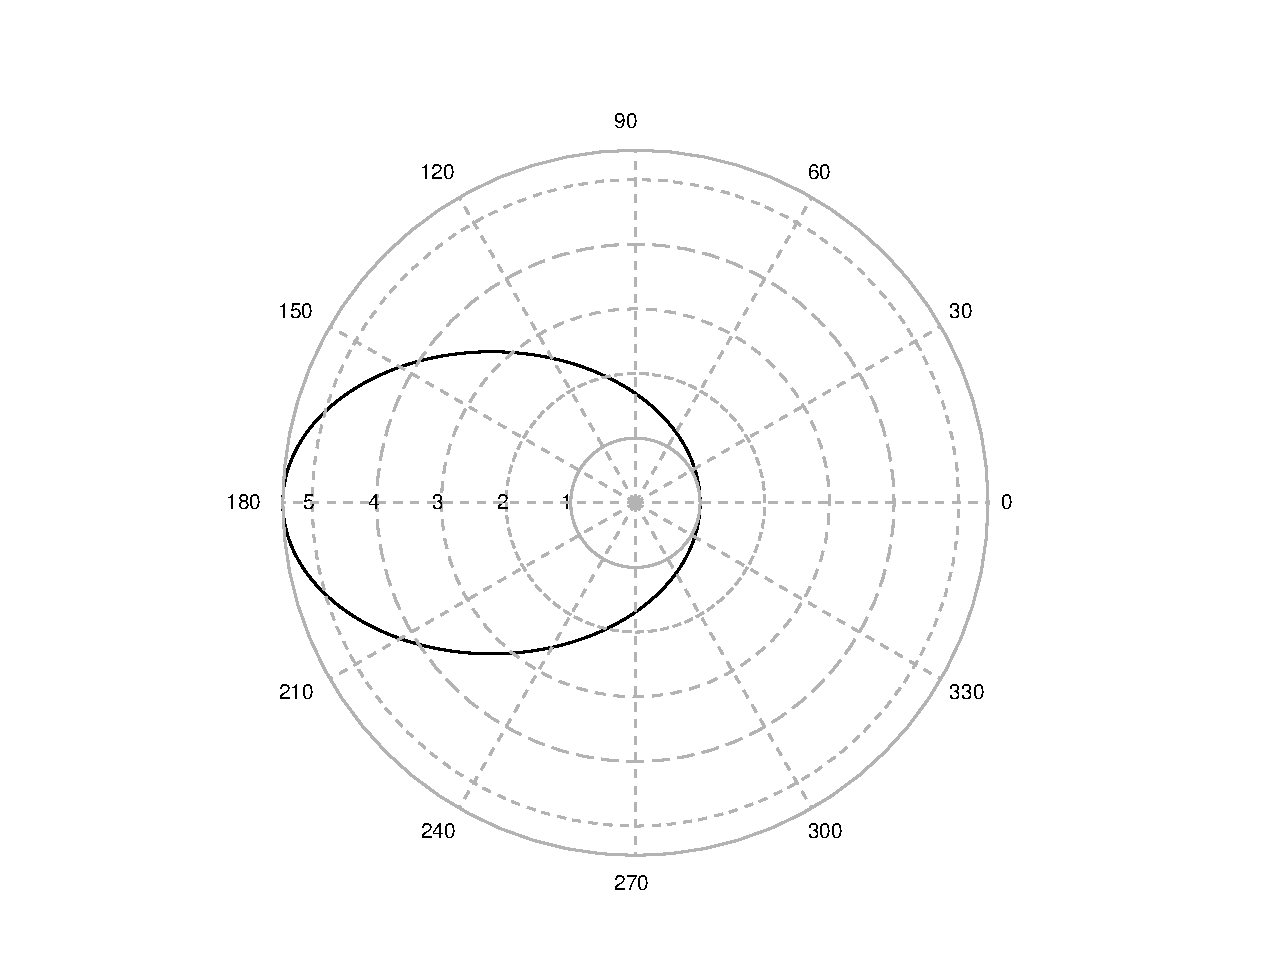
\includegraphics[scale=0.3]{ellipse.pdf}
		\label{flottants:precession:classique}}
		\subfloat[Corrected trajectory]{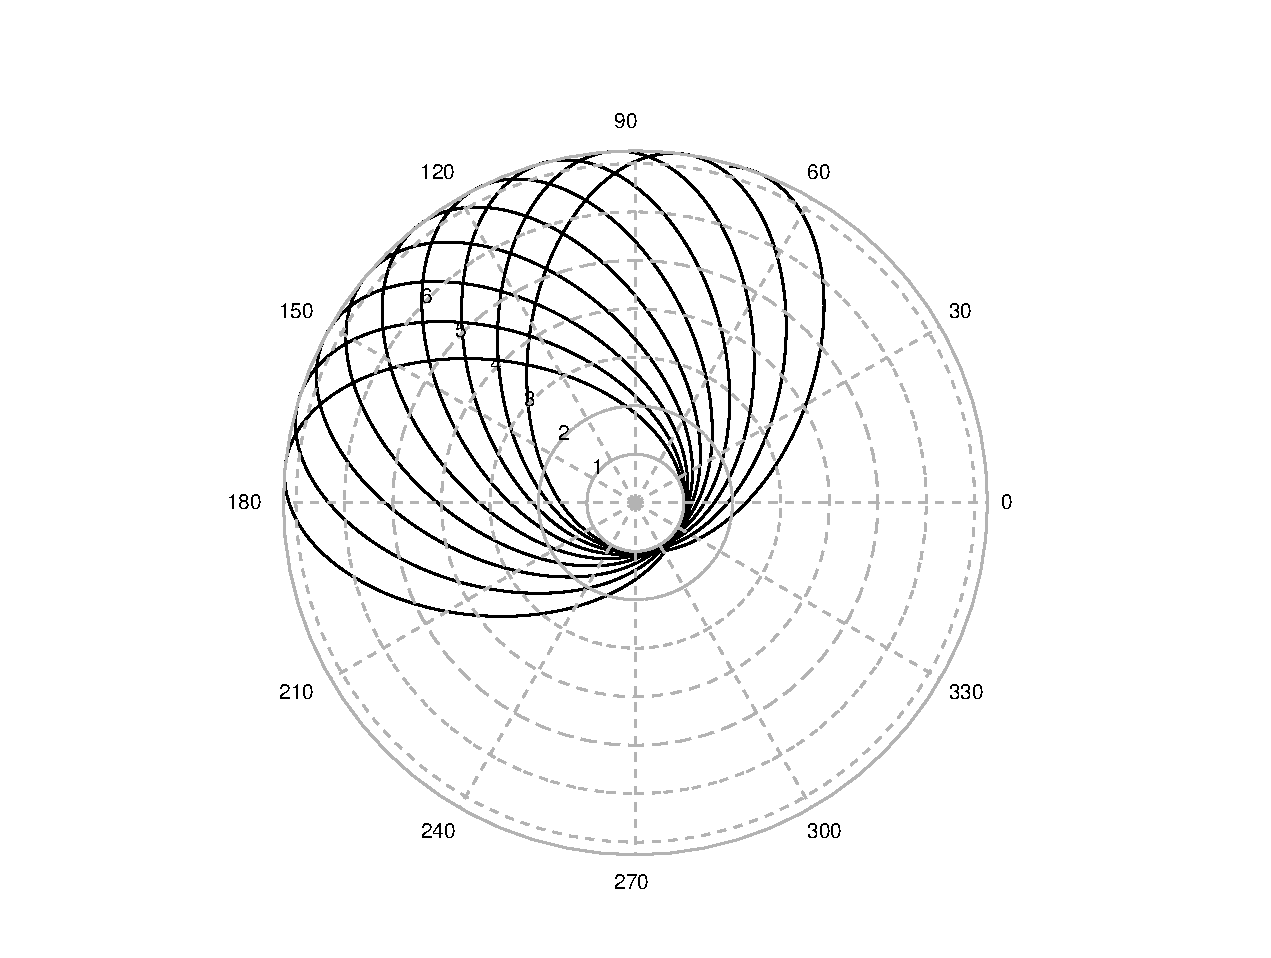
\includegraphics[scale=0.3]{precession.pdf}
		\label{flottants:precession:precession}}
	\end{center}
	\caption{We can see on these figures the differences between classic and corrected
	         trajectory. The first is a simple ellipse while the latter is an ellipse which
			 precess with time.}
	\label{flottants:precession:differences}
\end{figure}

\section{Conclusion}

In this project, we have seen how general relativity works and more particularly, we can
easily come back to the Newtonian theory by using some approximations or by removing simply
a part of a calculus. From this narrow link between these two theories, we also understood
that we could obtain better results by using the general relativity for problems than by
using gravitation.
Indeed, the fact that the empiric force defined by Newton centuries ago can be corrected by
a factor, allows us to apply the general relativity to some problems that Newtonian theory
could not resolve.
In our project, we have studied the perihelion precession of Mercury that can be only
understood by using general relativity, as the Newtonian theory predicts an invariable
ellipse.
However, this experiment is not the only one. There are many experimental justifications
confirming general relativity. For example, the redshift or the curvature of light rays.
And every time this approach passes the experimental test.

At the beginning of the project, we have planned to look for others solutions to Einstein
field equations. It might be also interesting to study another experiment to test the
general relativity or to compare the results that we have obtained by using another metric
of Einstein field equations like the Kerr metric. However, as the Schwarzchild metric has
already such a lot of interesting things, in the second part of our study, we changed to
looking for the application and the numerical simulation of the Schwarzchild metric, like
the perihelion precession of Mercury, in order to understand more clearly the correction
of Schwarzchild to Newton’s law. 

\newpage
\thispagestyle{empty}

\bibliographystyle{abbrv}
\nocite{*}
\bibliography{biblio}

\end{document}
